\documentclass[conference]{IEEEtran}

\usepackage{cite}
\usepackage{amsmath,amssymb,amsfonts}
\usepackage{algorithmic}
\usepackage{graphicx}
\usepackage{textcomp}
\usepackage{hyperref}
\usepackage{caption}
\usepackage{subcaption}
%\hypersetup{
%	
%	colorlinks = true
%	linkcolor = blue
%	filecolor = magenta
%	urlcolor = cyan		
%}


\def\BibTeX{{\rm B\kern-.05em{\sc i\kern-.025em b}\kern-.08em
    T\kern-.1667em\lower.7ex\hbox{E}\kern-.125emX}}

\begin{document}

\title{Judging a Book by it's Cover and Title\\}

\author{\IEEEauthorblockN{1\textsuperscript{st} Prathu Baronia \\ 14D070046}
\textit{Indian Institute of Technology, Bombay}\\
India
\and
\IEEEauthorblockN{2\textsuperscript{nd} Balraj Parmar \\ 14D070001}
\textit{Indian Institute of Technology, Bombay}\\
India
}

\maketitle

\begin{abstract}

Don't judge a book by it's cover is a common phrase in English which tells us not to evaluate a book from it’s cover page only. In this project we aim to do exactly this and show that it is possible to predict the genre of a book from the cover page art and the title of the book with a considerable accuracy.
Transfer Learning approach is used to extract features from the dataset using VGG-16 Convolutional Neural Network which was pretrained on the Imagenet Dataset. A simple neural network of three layers is trained using this features as input with a validation accuracy of 72.3\%. A Bag of words approach has been adopted to extract features from the book titles post pre-processing the dataset and a validation accuracy of 78.6\% was achieved through a Random Forest Classifier. 

\end{abstract}

\begin{IEEEkeywords}
component, formatting, style, styling, insert
\end{IEEEkeywords}

\section{Introduction}

The cover of the book is the first thing that we observe in a book. It is our first introduction to the book and along with the title functions to communicate to the reader about the style, tone and content of the book. Humans are naturally trained through their life experiences to guess the genre or the style of the book from the cover page and title with reasonable accuracy. In this project, we aim to train a model to predict the genre from the cover page and title using a Image Classifier and a Text Classifier. 

The difficulty of the task arises from the fact that there is a large variety in book covers and the title. Also, unlike many other classification problems where there the classes are more starkly defined, There is a lot of ambiguity about how a genre is defined and book covers are sometimes also intentionally misleading. There are innumerable books that have been written till now, and over the times there has been a lot of changes in how the genre is defined, the way artwork is used on the cover page to attract the viewer and so on. And so it’s important to select our data such that it can be a good representative of different genres, and which can be easily utilized by a Machine Learning model.

Convolutional Neural Networks(CNN) is a class of deep, feed-forward artificial neural networks that has successfully been applied to 0 visual imagery. They are the current state of the art method for image classification. But it has been observed that they generally require hundreds of thousands of images to perform accurately without over fitting. Transfer Learning has been suggested as one of the solution when our dataset is limited. It uses a CNN trained over millions of images to extract features( which are a good, compact representation of the data present in the images) and then use these features to train any classifier like a neural network or SVM etc.

We have used this approach in our solution. We have used VGG16\cite{b2} network pretrained on ImageNet database to extract features from our dataset, We have then created and trained a fully connected neural network on this features to classify our data in  five genres.

The bag-of-words model is a simplifying representation used in natural language processing and information retrieval (IR). Also known as the vector space model. In this model, a text (such as a sentence or a document) is represented as the bag (multiset) of its words, disregarding grammar and even word order but keeping multiplicity. The bag-of-words model has also been used for computer vision.
The bag-of-words model is commonly used in methods of document classification where the (frequency of) occurrence of each word is used as a feature for training a classifier.

\section{Related Works}

For the particular problem of genre prediction from book cover, Iwana et.al\cite{b3} compared custom LeNet\cite{b4} and pretrained AlexNet network for the genre classification problem. They found that  the Top-1 accuracy in the transfer learning approach with AlexNet was twice as good as the custom made LeNet network. They didn’t made use of the text titles of book at all. They relied only on images to predict the genre. 

Gatys et.al\cite{b5} have used deep CNNs to learn and copy the artistic style of paintings. There have been attempts at classifying music by genre, paintings and text. However, a large number of these methods use hand designed features.


% Theory and Approach

\section{Image Classification}

\subsection{Convolutional Neural Networks} 

Unlike traditional artificial neural networks for image classification which requires the image to be in a vectorized form (which results in loss of spatial information from the image), CNNs takes input in the matrix form (either 2D if it’s a gray scale or a binary image, or in multidimensional matrix in case of color spaces like RGB). CNNs comprises of three basic components: convolutional layers, pooling layers, and fully connected layers.

\begin{figure}[htbp]
\centerline{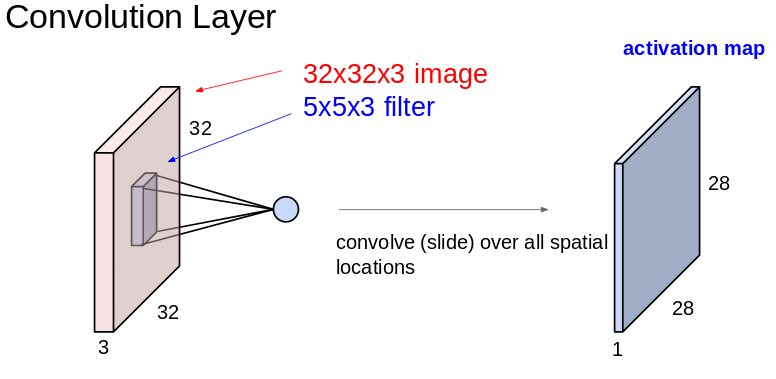
\includegraphics[width=0.5\textwidth]{pics/image_theory/clayer.png}}
\caption{ Unit of a convolution layer}
\label{figi:clayer}
\end{figure}%

\paragraph{Convolutional Layer\\}

The basic operation that gives the name to the model is the “convolution” operation. An important feature of CNNs which helps in minimizing the number of parameters compared to a Fully Connected Network of similar architecture is the idea of “weight sharing”. All the neurons/kernels in a particular convolutional layer have the same weights which are learned during training. The output of this layer would be equivalent to what you get if you would have convolved the input matrix with a kernel equivalent to one of the neurons. 

\paragraph{Pooling Layer\\}
Another important feature of CNNs is it’s pooling layer, it is a down-sampling operation which serves two purposes: it helps in reducing number of parameters(and hence amount of computation) and it helps in firming the fact that the exact location of a particular value in the feature map is less important. 

\begin{figure}[htbp]
\centerline{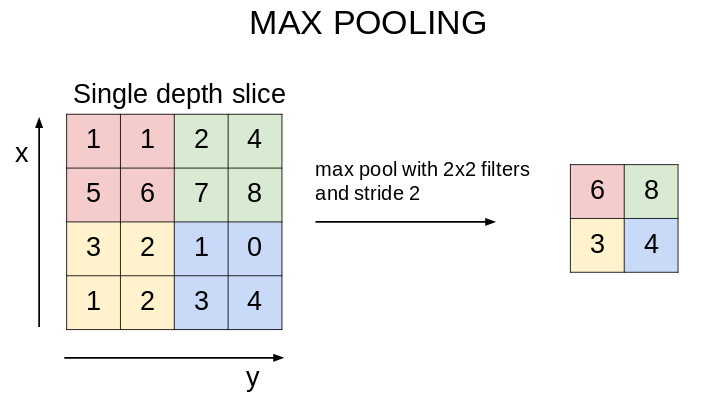
\includegraphics[width=0.5\textwidth]{pics/image_theory/max_pool.png}}
\caption{ Max Pooling}
\label{fig:pooling}
\end{figure}%


\paragraph{Fully Connected Layer\\}

All the neurons in this layer are connected to all the neurons in the previous layer just like a traditional neural network architecture.
\begin{figure}[htbp]
\centerline{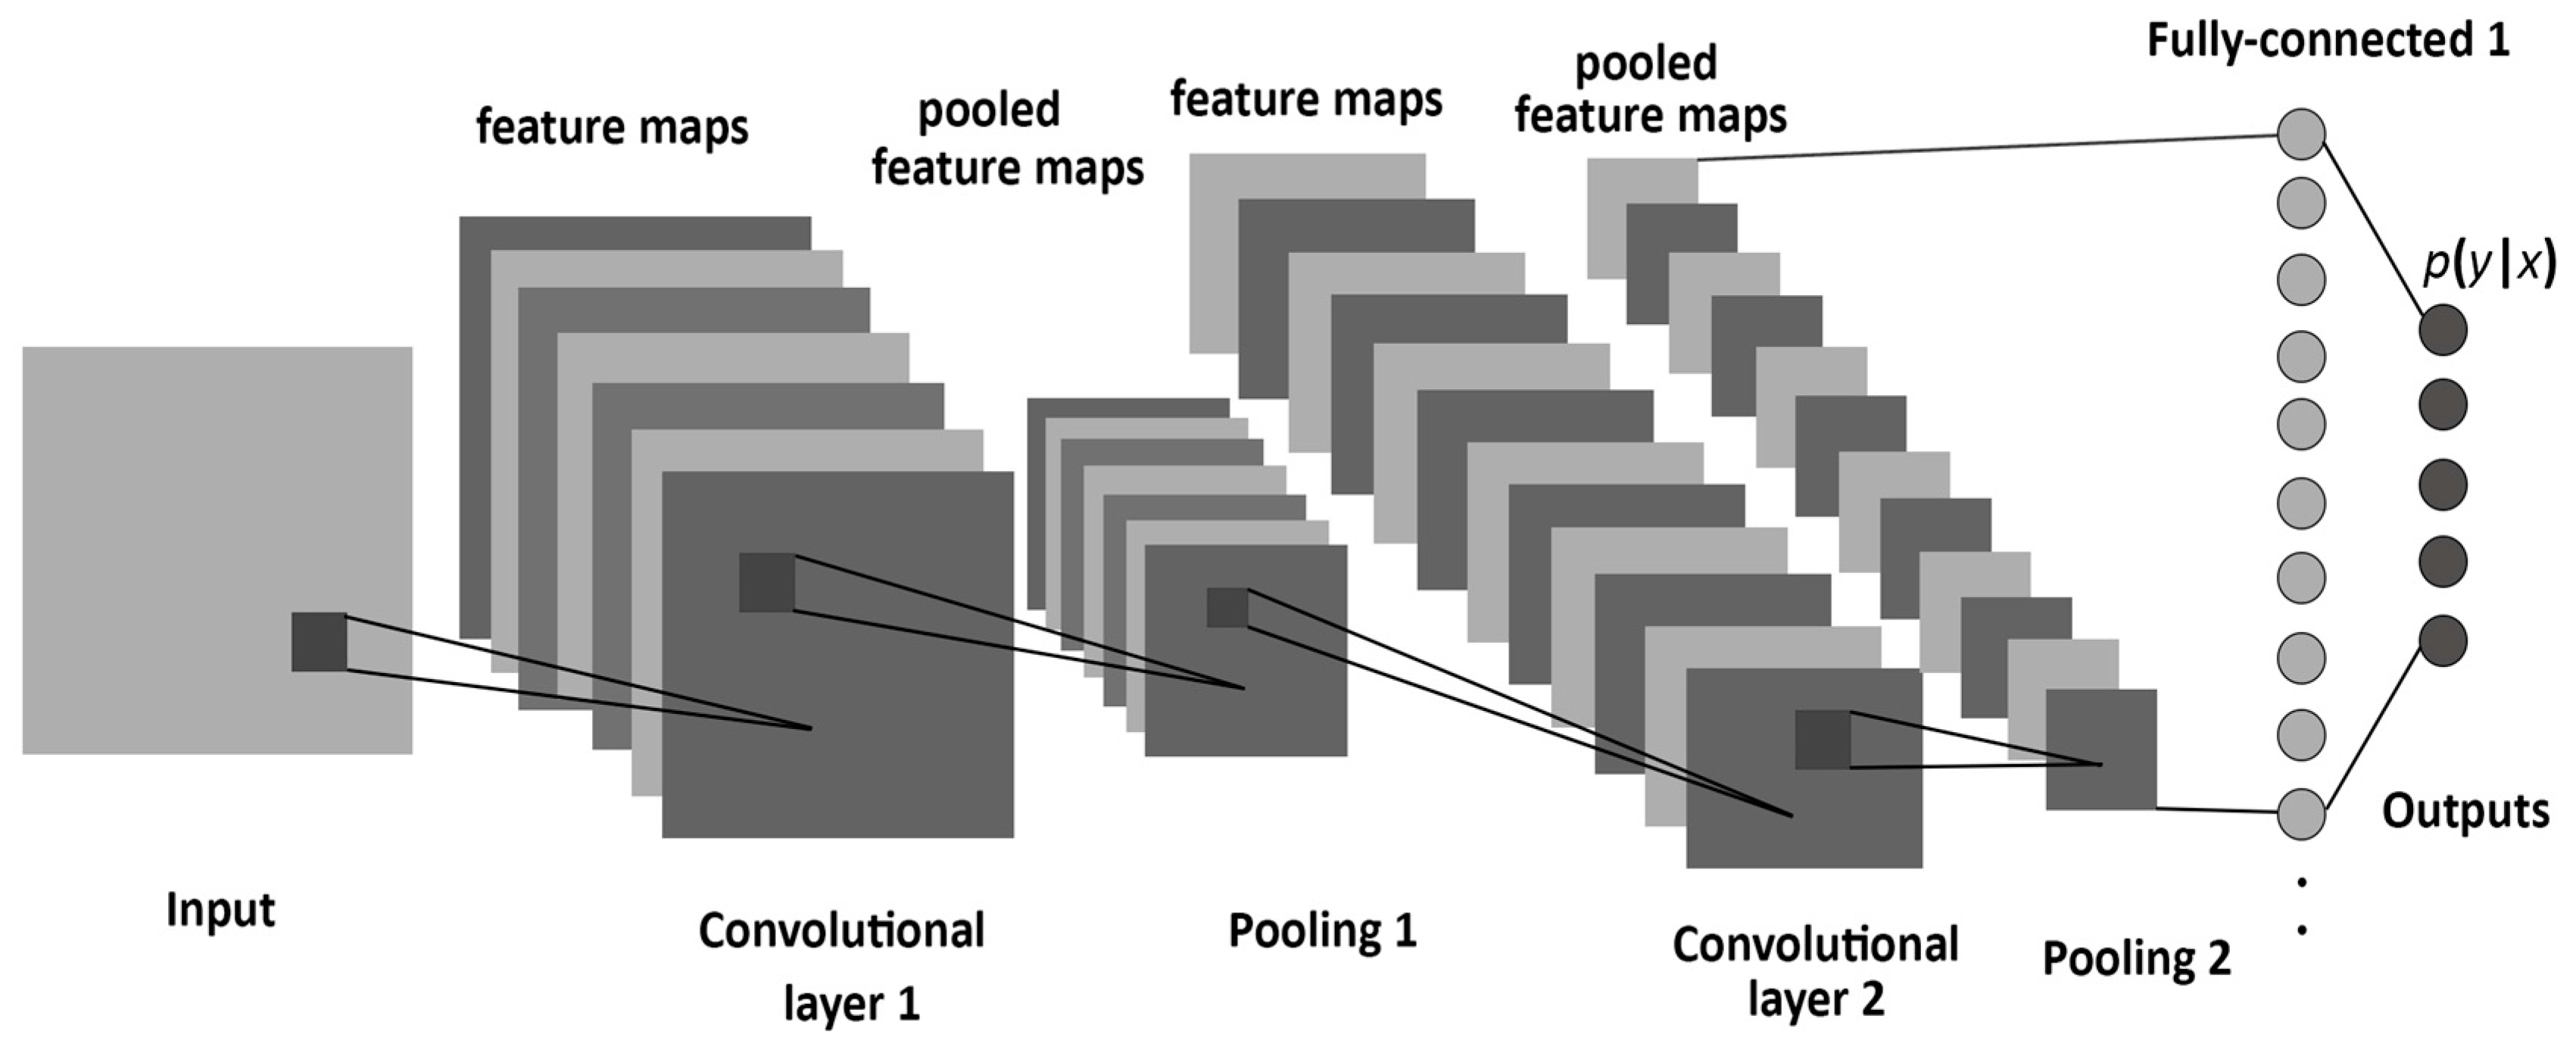
\includegraphics[width=0.5\textwidth]{pics/image_theory/cnn.png}}
\caption{ Fully connected layer in a CNN}
\label{fig:cnn}
\end{figure}%

\paragraph{Activation Functions\\}

As far as activation functions are concerned, Activation functions like sigmoid and tanh suffered from the problem of vanishing gradients and the training time increased. Recently, ReLu (Rectified Linear Unit) (ReLu(x) = max(0, x)) has been the most favorable activation function among researchers owing to the fact that it speeds up the training time significantly without deteriorating the accuracy. 

The CNNs have been back in limelight after AlexNet\cite{b1} showed remarkable performance in ImageNet challenge 2012. 

\subsection{Transfer Learning}
One caveat when using CNNs is that, it often requires hundred of thousands of training samples to give good accuracy without over fitting. But often we find that, our dataset has only few hundred or thousand samples. Transfer Learning has been suggested as one of the methods to use in such scenarios. It has been found that features learned by a deep CNNs on one dataset of images with millions of images are highly transferable to another problem. This is especially true for natural images. So a pretrained network is used to extract features and these features are used to train a classifier like a neural network or SVM.


\subsection{VGG16 network}
VGG16 network’s philosophy is uniformity and deep layers. It uses a uniform 3x3 filters in all the layers. It showed that increasing the depth indeed results in better performance over ImageNet dataset. A 16 layer and a 19 layer version are publically available for academic use.

\begin{figure}[htbp]
\centerline{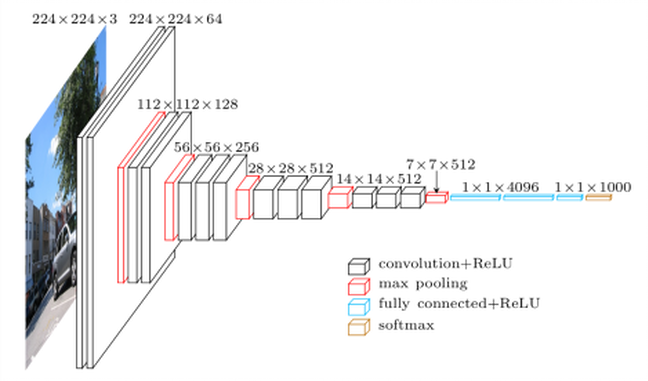
\includegraphics[width=0.5\textwidth]{pics/image_theory/vggnet.png}}
\caption{ Architecture of VGGNet }
\label{fig:vggnet}
\end{figure}%

Here in our solution to the problem, we have used pretrained VGG16 network to extract features from our dataset. A three layer network is then trained using these features to classify into 5 genres.


\section{Bag of Words}

A problem with modeling text is that it is messy, and techniques like machine learning algorithms prefer well defined fixed-length inputs and outputs.
Machine learning algorithms cannot work with raw text directly; the text must be converted into numbers. Specifically, vectors of numbers.In language processing, the vectors x are derived from textual data, in order to reflect various linguistic properties of the text.This is called feature extraction or feature encoding.
A popular and simple method of feature extraction with text data is called the bag-of-words model of text.

A bag-of-words is a representation of text that describes the occurrence of words within a document. It involves two things:
\begin{itemize}
	\item A vocabulary of known words.
	\item A measure of the presence of known words.
\end{itemize}
It is called a “bag” of words, because any information about the order or structure of words in the document is discarded. The model is only concerned with whether known words occur in the document, not where in the document. 
The intuition is that documents are similar if they have similar content. Further, that from the content alone we can learn something about the meaning of the document.The bag-of-words can be as simple or complex as you like. The complexity comes both in deciding how to design the vocabulary of known words (or tokens) and how to score the presence of known words.
\subsection{Example of Bag of Words}

\begin{table}[hbtp]
\caption{Example Sentences}

\begin{center}

\begin{tabular}{|c|}

\hline
It was the best of times,\\
it was the worst of times,\\
it was the age of wisdom,\\
it was the age of foolishness,\\
\hline

\end{tabular}

\label{tab1}
\end{center}

\end{table}

Here in TABLE \ref{tab1} we present a set of example sentences taken from a popular book.\\
Vocabulary is the list of unique words in the input. Here the vocabulary is : \{ 'it', 'was', 'the', 'best', 'of', 'times', 'worst', 'age', 'wisdom', 'foolishness'\}

The objective is to turn each document of free text into a vector that we can use as input or output for a machine learning model.
Because we know the vocabulary has 10 words, we can use a fixed-length document representation of 10, with one position in the vector to score each word.
The simplest scoring method is to mark the presence of words as a boolean value, 0 for absent, 1 for present. 

\begin{table}[hbtp]
\caption{Encoded Sentences}

\begin{center}

\begin{tabular}{|c|}

\hline
$$ [ 1, 1, 1, 1, 1, 1, 0, 0, 0, 0 ] $$ \\
$$ [ 1, 1, 1, 0, 1, 1, 1, 0, 0, 0 ] $$ \\
$$ [ 1, 1, 1, 0, 1, 0, 0, 1, 1, 0 ] $$\\
$$ [ 1, 1, 1, 0, 1, 0, 0, 1, 0, 1 ] $$\\
\hline

\end{tabular}

\label{tab2}
\end{center}

\end{table}

In \ref{tab2} we present encoded sentences which we can input to a classifier for training and testing purposes.

\section{Implementation}

\subsection{Image Classifier}

\begin{figure}[htbp]
\centerline{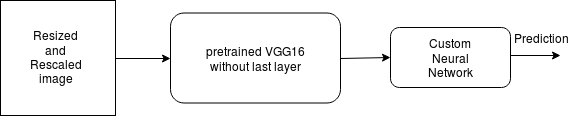
\includegraphics[width=0.5\textwidth]{pics/block_images/image.png}}
\caption{ Image Classifier Flow }
\label{fig:imageflow}
\end{figure}%


\paragraph{Dataset\\}

Our dataset was downloaded from \cite{b7}. The dataset initially had a lot of faulty images. Some were empty, some weren’t originally in the jpeg format but were forcibly were stored at .jpeg which resulted in an error when those were read by the code. There were also some images in formats which weren’t supported by the module. Our Dataset after this process had total 30000+ images(~6000 images per class) which were separated into 80\% training set and 20\% validation set.

\paragraph{Model\\}

Input images are resized to 150 $\times$ 150 size. The are also normalized so that the image intensity values lies in the range 0 to 1. These pre-processed image is then passed to VGG Network. 
Features are extracted from the second last layer of VGGNet. These features are then used to train a neural network of three layers. Number of neurons in the first layer are 256, number of neurons in the second layer are 128, number of neurons in the final(classification) layer are 5. Dropout of 0.5 is used to prevent over fitting. RMSProp is used as the optimizer. Sparse Categorical Cross Entropy is used as the loss function. Relu is used as the activation for intermediate layer. Softmax is used for the classification layer.
While testing on a new image, the image is passed to the preprocessing part. It is then passed to VGGNet to extract features. These features are then used as input to the trained neural network and it is classified in one of the genres.

\paragraph{Resource used for training\\}
A VM instance was created on Google Cloud. We weren’t able to get an access to GPU which hindered the progress and limited the scope of our project to some access. Google Cloud helped us to some extent but wasn’t as efficient as expected. 

\paragraph{Modules\\}
The code was written in Python3. The code structure was adopted from \cite{b8} \\
 Module dependencies: Tensorflow, Keras, Numpy, h5py

\subsection{Text Classifier}

\begin{figure}[htbp]
\centerline{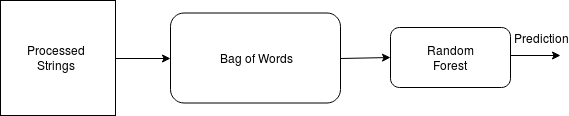
\includegraphics[width=0.5\textwidth]{pics/block_images/text.png}}
\caption{ Text Classifier Flow }
\label{fig:textflow}
\end{figure}%


Starting off with pre-processing, the dataset contained a lot of blank spaces which had to be replaced with \emph{numpy.nan} so that the classifier can identify it as a NaN value. For Bag of Words implementation the sklearn module of python has inbuilt Vectorizers which allows the user to convert the input title strings into numerical binary arrays. Here we have used the \textbf{Count Vectorizer} which after initialization needs to be fitted to the input string list before transforming it into a binary array. After obtaining a binary array out of the titles we input them to a \textbf{Random Forest Classifier} with a parameter value of 100 which implies a forest of 100 trees.

\paragraph{Modules\\}
The code as been written in Python.\\
Module dependencies : Numpy, Sklearn, Pandas

\section{Results \& Discussion}

%\begin{figure}[htbp]
%\centerline{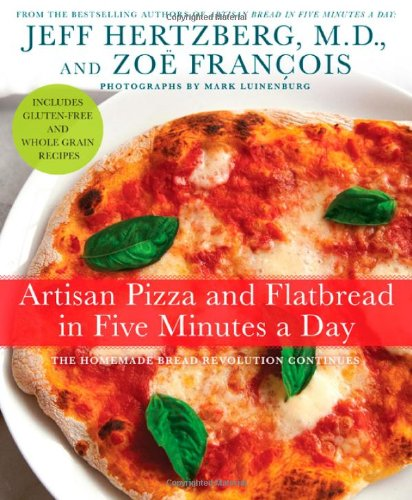
\includegraphics[scale=0.2]{pics/results_image/0.jpeg}}
%\caption{Cookbook, Food \& Wine }
%\label{fig:cookbook}
%\end{figure}%
%
%\begin{figure}[htbp]
%\centerline{
\includegraphics[scale=0.2]{pics/results_image/1.jpeg}}
%\caption{Romance }
%\label{fig:romance}
%\end{figure}%
%
%\begin{figure}[htbp]
%\centerline{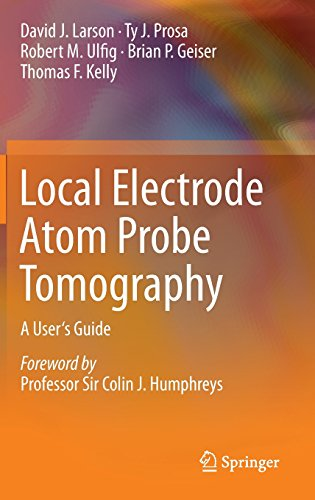
\includegraphics[scale=0.2]{pics/results_image/2.jpeg}}
%\caption{ Science \& Math }
%\label{fig:science}
%\end{figure}%
%
%\begin{figure}[htbp]
%\centerline{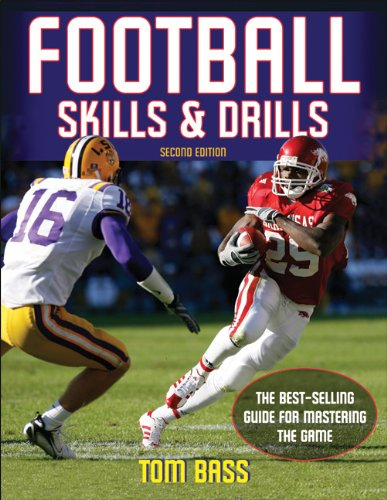
\includegraphics[scale=0.2]{pics/results_image/3.jpeg}}
%\caption{Sports \& Outdoors}
%\label{fig:sports}
%\end{figure}%
%
%\begin{figure}[htbp]
%\centerline{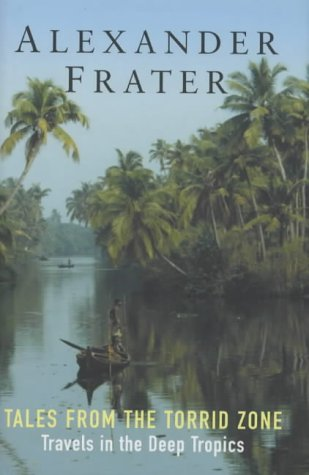
\includegraphics[scale=0.2]{pics/results_image/4.jpeg}}
%\caption{Travel}
%\label{fig:travel}
%\end{figure}%

\subsection{Image Classifier}

\begin{table}[hbtp]
\centering
\caption{Test Samples for Cookbook,\\ Romance, Science, Sports \& Travel in clockwise order}

\begin{center}

\begin{tabular}{c c c}
  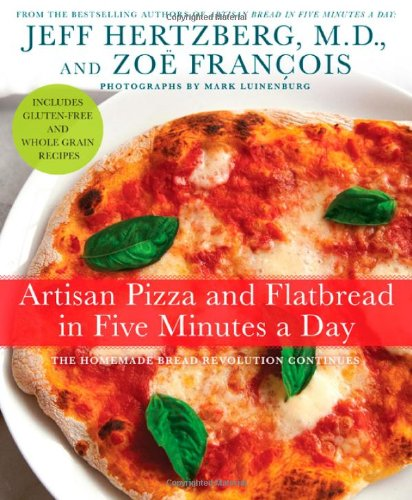
\includegraphics[scale=0.2]{pics/results_image/0.jpeg} &
  
\includegraphics[scale=0.2]{pics/results_image/1.jpeg} &
  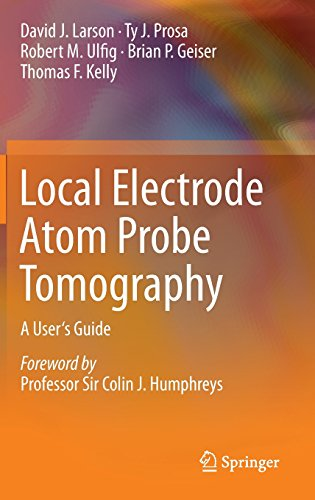
\includegraphics[scale=0.2]{pics/results_image/2.jpeg} \\
  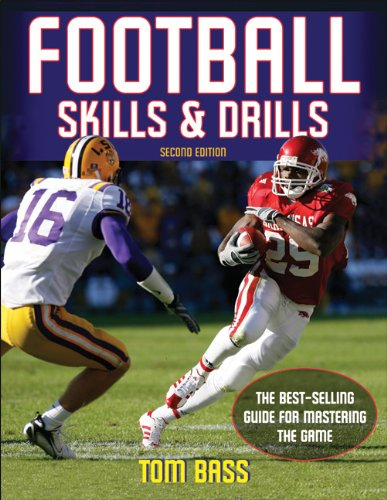
\includegraphics[scale=0.2]{pics/results_image/3.jpeg} &
  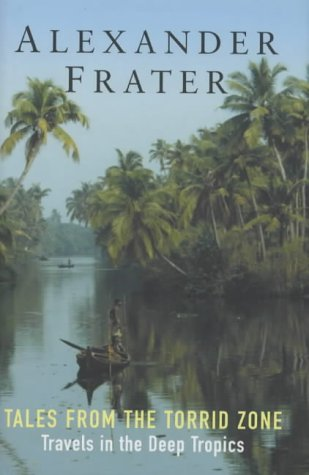
\includegraphics[scale=0.2]{pics/results_image/4.jpeg} \\ 

  \end{tabular}
\end{center}
\label{testtab}
\end{table}

\begin{table}[hbtp]
\centering
\caption{Misclassified Samples for Cookbook,\\ Romance, Science, Sports \& Travel in clockwise order}

\begin{center}

\begin{tabular}{c c c}
  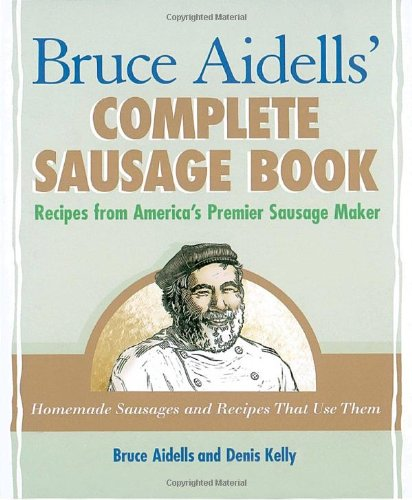
\includegraphics[scale=0.2]{pics/non_results_images/food.jpeg} &
  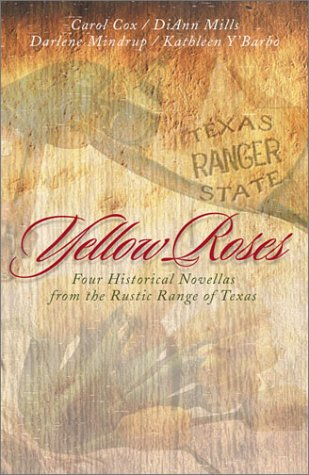
\includegraphics[scale=0.2]{pics/non_results_images/romance.jpeg} &
  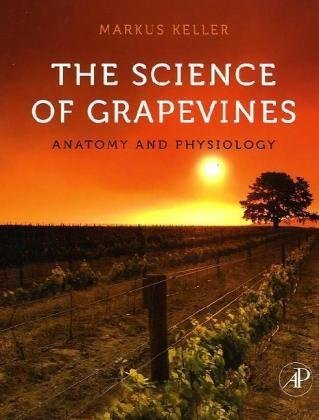
\includegraphics[scale=0.2]{pics/non_results_images/science.jpeg} \\
  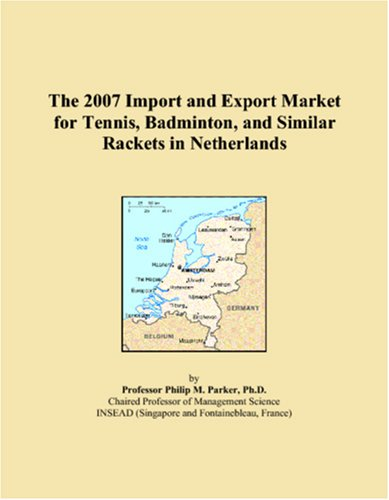
\includegraphics[scale=0.2]{pics/non_results_images/sports.jpeg} &
  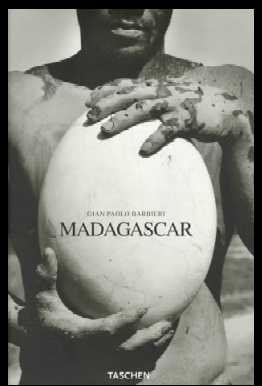
\includegraphics[scale=0.2]{pics/non_results_images/travel.jpg} \\ 

  \end{tabular}
\end{center}
\label{nontesttab}
\end{table}

We observed a training accuracy of 75\% and a validation accuracy of 69.04\% on the dataset. 
Some of the misclassification happened because of the vagueness in the cover. For example in TABLE \ref{nontesttab} the Food figure, in it there is no indication of a food item and perhaps due to presence of a human in a particular pose(which is prevalent in sports biographies) it is classified as Sports \& Outdoors instead of Cookbooks,Food, and Wine.
Simple, plain covers with few text have a tendency to be classified as Science \& Math. This type of problem is seen in the case of the romance figure in TABLE \ref{nontesttab}.
In case if a natural scenery is present in the image like mountains, sunrise, ice, forest etc, Then the image has tendency to be classified as Travel. This can be seen in the science figure, which actually belongs to Science \& Math but is classified as Travel.
For sports figure, the presence of a person without clothes perhaps in a posture forces it to be categorized as Romance instead of Travel. 
It’s clear from the misclassified images that the machine is able to predict what an average human would have done on observing the cover. We are able to show that the machine can be trained to come closer to human level performance on this problem.

%input 
\begin{table}[hbtp]
\caption{Input to Text Classifier}
\begin{center}
\begin{tabular}{c|p{5cm}}
\textbf{Category} & \textbf{Title} \\
\hline
Sports \& Outdoors	&	Sports Training Notebook: Badminton: For Coaching Instruction On All Levels Of Sport \\
\hline
Travel			&	Antarctica Satellite (Laminated) (National Geographic Reference Map) \\
\hline
Travel			&	Eyes to See: U.S. Volunteers in Nicaragua \\
\hline
Cookbooks, Food \& Wine	&	Pizza, A Slice of American History \\
\hline
Cookbooks, Food \& Wine	&	Build Your Own underground Root Cellar \\
\hline
Cookbooks, Food \& Wine	&	Brown Eggs and Jam Jars: Family Recipes from the Kitchen of Simple Bites \\
\hline
Travel			&	Aruba 1:50,000 \& Oranjestad 1:10 000 Travel Map, waterproof, BORCH \\
\hline
Sports \& Outdoors	&	The Fundamentals of Hogan \\
\hline
Sports \& Outdoors	&	Alone: The Triumph and Tragedy of John Curry \\
\hline
Travel			&	Virgin Islands Reef Creatures Guide Franko Maps Laminated Fish Card 4" x 6" \\
\end{tabular}
\label{tab4}
\end{center}
\end{table}

\subsection{Text Classifier}
Inputs to the classifier have been presented in TABLE \ref{tab4} in the form of book title and the corresponding book genre. TABLE \ref{tab5} shows the output of the classifier and as can be seen that the classifier predicts the genre labels perfectly because of the small size of the test dataset. When tested fora large dataset i.e 20,000 labels we get a validation accuracy of $\approx 79 \% $.


%output
\begin{table}[hbtp]
\centering
\caption{Output of Text Classifier}
\begin{center}
\begin{tabular}{c|p{5cm}}
\textbf{Category} & \textbf{Title} \\
\hline
Sports \& Outdoors	&	Sports Training Notebook: Badminton: For Coaching Instruction On All Levels Of Sport \\
\hline
Travel			&	Antarctica Satellite (Laminated) (National Geographic Reference Map) \\
\hline
Travel			&	Eyes to See: U.S. Volunteers in Nicaragua \\
\hline
Cookbooks, Food \& Wine	&	Pizza, A Slice of American History \\
\hline
Cookbooks, Food \& Wine	&	Build Your Own underground Root Cellar \\
\hline
Cookbooks, Food \& Wine	&	Brown Eggs and Jam Jars: Family Recipes from the Kitchen of Simple Bites \\
\hline
Travel			&	Aruba 1:50,000 \& Oranjestad 1:10 000 Travel Map, waterproof, BORCH \\
\hline
Sports \& Outdoors	&	The Fundamentals of Hogan \\
\hline
Sports \& Outdoors	&	Alone: The Triumph and Tragedy of John Curry \\
\hline
Travel       		&	Virgin Islands Reef Creatures Guide Franko Maps Laminated Fish Card 4" x 6" \\
\end{tabular}
\label{tab5}
\end{center}
\end{table}

\section{Conclusion \& Future Work}
We conclude that it’s possible to predict the genre of the book from it’s cover and the title. As expected, the text classifier performed better than the image classifier because of less ambiguity in the titles compared to the cover art. 

For image classification, we might want to try ResNet or InceptionNet CNNs to get the feature vectors for training in future as they show better performance on ImageNet compared to VGGNet which was used here. We can also ensemble the text and image classifiers by using something like mixture of experts model or a softmax gating network. It’s expected that the ensemble will show better performance than the individual classifiers. 

For text classification we might want to try Hash Vectorizer or TfIdf Vectorizer to increase the speed and to consume less memory space.
%\pagebreak
\begin{thebibliography}{00}
\bibitem{b1} Krizhevsky et.al, ImageNet Classification with Deep Convolutional Neural Networks, 2012 
\bibitem{b2} Simonyan et.al, Very Deep Convolutional Networks for Large-Scale Image Recognition, 2014 
\bibitem{b3} Iwana et.al, Judging a Book by it’s cover, 2016 
\bibitem{b4} LeCun et.al, Gradient-Based Learning Applied to Document Recognition, 1998 
\bibitem{b5} Gatys et.al, A neural algorithm of artistic style, 2015
\bibitem{b6} Bay Area Deep Learning presentation by Andrej Karpathy
\bibitem{b7} \href{https://github.com/uchidalab/book-dataset}{Link to the Dataset}
\bibitem{b8} \href{https://blog.keras.io/building-powerful-image-classification-models-using-very-little-data.html}{Keras tutorial}
\bibitem{b9} \href{https://keras.io/applications/}{Info on Pretrained Networks and their usage}
\bibitem{b10} \href{https://machinelearningmastery.com/gentle-introduction-bag-words-model/}{Bag of Words Tutorial} 
\bibitem{b11} \href{https://en.wikipedia.org/wiki/Convolutional\_neural\_network}{CNN Wiki}
\bibitem{b12} \href{https://en.wikipedia.org/wiki/Bag-of-words\_model}{Bag of Words Wiki}
\end{thebibliography}

\end{document}
